\documentclass[a4paper]{article}

%% Language and font encodings
\usepackage[english]{babel}
\usepackage[utf8x]{inputenc}
\usepackage[T1]{fontenc}


%% Sets page size and margins
\usepackage[a4paper,top=3cm,bottom=2cm,left=3cm,right=3cm,marginparwidth=1.75cm]{geometry}

%% Useful packages
\usepackage{amsmath}
\usepackage{graphicx}
\usepackage{tikz,pgfplots}
\usepackage[colorinlistoftodos]{todonotes}
\usepackage[colorlinks=true, allcolors=blue]{hyperref}
\usepackage{amsfonts}
\usepackage{bbm}
\usepackage{dsfont}
\usepackage{cancel}
\usepackage{tikz,tkz-base,tkz-fct}
\newcommand{\prob}{\mathbb{P}}
\newtheorem{definicion}{Definición}
\newtheorem{teorema}{Teorema}
\newtheorem{ejemplo}{Ejemplo}
\DeclareMathOperator*{\argmax}{Arg\,max}
\newtheorem{lem}{Lemma}
\newtheorem{prop}{Proposici\'on}
\newtheorem{cor}{Corolario}
\newtheorem{dem}{Demostración}
\numberwithin{equation}{subsection}
\newtheorem{obs}{Observación}


%% Aquí se pueden definir nuevas abreviaturas para algunos comandos

\def\sen{{\rm sen\mspace{1.5mu}}}
\def\C{\mathbb C}
\def\R{\mathbb R}
\def\N{\mathbb N}
\def\Q{\mathbb Q}
\def\Z{\mathbb Z}
\def\V{\mathbb V}
\def\E{\mathbb E}
\def\to{\rightarrow}
\newcommand{\pb}{\mathbb{P}}



\newcommand{\ds}{\displaystyle}


%Para hacer normas en tex

\providecommand{\norm}[1]{\lVert#1\rVert}
\providecommand{\normm}[1]{\bigg\lVert#1\bigg\rVert}


%integrales bacanes
\usepackage{ esint }

%Para poner en negrita en modo matemático
\newcommand{\negri}{\boldsymbol}




\title{Simulación Estocástica}
\author{Clase 3}
\date{5 de agosto de 2019}

\begin{document}
\maketitle

\section{Notación}
\begin{itemize}
    \item \textbf{T.C.D.}: "Teorema de convergencia  dominada".
    \item $\mathcal{N}(\mu,\sigma)$: "Distribución normal de media $\mu$ y desviación estándar de $\sigma$", se hará un abuso de notación ya que también simbolizará la variable aleatoria que distribuya de esta forma.
\end{itemize}

\subsection{Tensión (Tightness)}
\subsubsection{Relativamente compacto.}
Sea $M\subset \mathcal{P}(E)$ una familia de medidas de probabilidad sobre el espacio métrico $(E,d)$. Diremos que $M$ es \textit{relativamente compacto} si cada sucesión de elementos en $M$ contiene una subsucesión que converge débilmente, es decir; si $\{\mu_n\}$ es una secuencia de elementos en $M$, entonces existe una subsucesión $\{\mu_{n_i}\}$ y una medida de probabilidad $\mu \in \mathcal{P}(E)$, tal que $\mu_{n_i} \Rightarrow \mu$.  \\ \newline
Notamos que esta caracterización evita la descripción topológica que se encuentra subyacente en las definiciones de \textit{compacidad} o \textit{convergencia}. Se puede mostrar la existencia de una métrica que dota al espacio de tal topología pero no es de vital importancia para este curso, he ahí el motivo de su ausencia en estas notas. \\ \newline
Sin embargo, notamos que esta definición genera cierto problema para probar que un conjunto de medidas es relativamente compacto, dada la escasa gama de herramientas que poseemos en este momento. Es por esto, que se introduce la siguiente definición:

\begin{definicion}[Tensión] Una familia $M\subseteq \mathcal{P}(E)$ se dice \textbf{TENSA} si $\forall \epsilon > 0$, $\exists K\subseteq E$ compacto tal que:
\[\mu(K) > 1-\epsilon \hspace{1cm}\forall\,\mu\in M\]
\end{definicion}
\\ \newline
El siguiente resultado importante justifica la definición anterior:


\begin{teorema}[de Prohorov] Sea $M\subseteq \mathcal{P}(E)$.
\begin{itemize}
    \item[i)] Si $M$ es tensa, entonces es relativamente compacta.
    \item[ii)] Supongamos que $E$ es un espacio \textbf{polaco} (espacio métrico completo y separable). Si $M$ es relativamente compacta, entonces es tensa.
\end{itemize}
\end{teorema}
Antes de demostrar este teorema anunciaremos el siguiente corolario.

\begin{cor} Si $\{\mu_n\}$ es tensa y cada subsucesión débilmente convergente, converge a la misma medida $\mu\in\mathcal{P}(E)$, entonces toda la secuencia $\mu_n$ converge débilmente a $\mu$: $\mu_n \Rightarrow \mu$.
\end{cor}

\begin{ejemplo}
\begin{itemize}
    \item Si $E$ es compacto, entonces toda familia $M\subseteq \mathcal{P}(E)$ es tensa.
    \item En $E=\R$, sea $M=\{\delta_n \}$ el conjunto de las delta de Dirac en los puntos $n\in\N$. Claramente $M$ no es tensión, cada vez que proponemos un conjunto compacto, al ser la sucesión \\$\{n\,|\, n\in\N\}$ no acotada, existirá un $n$ suficientemente grande que se escape del compacto en $\R$. 
    \item En $E=\R$, sea $M=\{\mathcal{N}(0,n)\}_{n\in\N}$. $M$ no es tensión.
\newpage
\begin{figure}[h!]
\centering
    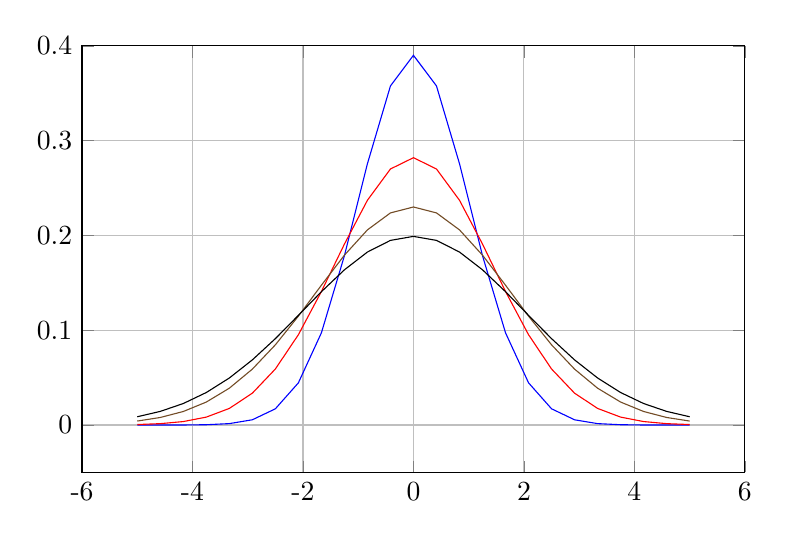
\begin{tikzpicture}
         \begin{axis}
        [width=10cm, height=7cm, xmin=-6, xmax=6, ymin=-0.05, ymax=0.4, xmajorgrids=true, ymajorgrids=true, xtick={-6,-4,-2,0,2,4,6},  xticklabels={-6,-4,-2,0,2,4,6}, ytick={0,0.1,0.2,0.3,0.4}, yticklabels={0,0.1,0.2,0.3,0.4}]
        
        \addplot+[no marks]{0.39*e^(-0.5*x^2)};
        \addplot+[no marks]{0.282*e^(-0.25*x^2)};
        \addplot+[no marks]{0.23*e^(-0.16*x^2)};
        \addplot+[no marks]{0.199*e^(-0.125*x^2)};
        \end{axis}
    \end{tikzpicture}
    \caption{Sucesión de densidades $\mathcal{N}(0,n)$.}
\end{figure}

    \item Sin embargo, considerando $E=\overline{\R}:=\R\cup \{-\infty ,+\infty\}$, entonces la sucesión $M=\{\delta_n \}_n$ es tensa pues: $\delta_n \Rightarrow \delta_{+\infty}$.
    
    \item De la misma forma, si $E=\overline{\R}$, la familia de medidas $M=\{\mathcal{N}(0,n)\}_n$, entonces:
    \[\mathcal{N}(0,n) \Rightarrow\,\frac{1}{2}\,\delta_{-\infty} + \frac{1}{2}\,\delta_{+\infty}\]
\end{itemize}
\end{ejemplo}

\section{Función Característica}
Son variadas las transformaciones o funciones generadoras usadas en matemáticas, probabilidades y estadística. En general, todas ellas se basan en el uso de la función exponencial y su ventaja de convertir sumas en productos. En la siguiente sección se denotará como $i$ $(=\sqrt{-1})$ a la componente imaginaria de un valor complejo.\\
Los siguientes son ejemplos de transformadas o funciones del tipo antes mencionado:
\begin{enumerate}
    \item Función generadora de probabilidades: $g(s)=\E(s^{X})$
    \item Función generadora de momentos: $m(t) = \E(e^{tX})$
    \item Transformada de Laplace: $\mathbb{L}(t) = \E(e^{-tX}) = \int e^{-tx}\mu(dx)$
    \item Transformada de Fourier: $\E(e^{-itX}) = \int e^{-itx}\mu(dx)$
\end{enumerate}

En lo que sigue, nuestro espacio de trabajo será el espacio métrico $\R$ o $\R^{d}$ dotados de las métricas usuales.

\begin{definicion}[Función Característica] Dada $\mu \in \mathcal{P}(\R^{d})$, definimos su FUNCION CARACTERÍASTICA como:

    \[\hat{\mu}:\,\R^{d} \longrightarrow\,\C\]
    \begin{equation}
    t \longrightarrow \hat{\mu}(t) := \int_{\R^d} e^{it\cdot x}\mu(dx)
\end{equation}
Donde la notación:
\[t\cdot x = \sum_{j=1}^{d}t_j x_j\]
\end{definicion}

Equivalentemente, podemos enunciar la definición anterior para variables aleatorias, donde la función característica de la variable está dada por la función característica de su ley.

\begin{definicion} Dada $X$, variable aleatoria en $\R^d$, su FUNCIÓN CARACTERÍSTICA es:
\[\varphi_X(t):\R^d \longrightarrow\,\C\]
\begin{equation}
    t \,\longrightarrow\,\varphi_X(t) := \E(e^{it \cdot X})
\end{equation}
\end{definicion}
\begin{obs} Podemos notar que la función característica toma valores en el plano complejo, sin embargo; su cálculo se efectúa sólamente en variables reales.
\[\varphi_X(t) = \E(e^{itX}) = \int e^{itx}\mu(dx) = \E(cos(tX)) + i\,\E(sen(tX))\]
\end{obs}

\begin{ejemplo}
 $X\sim \mathcal{N}(\mu,\sigma^{2})$, donde, en este caso, $\mu$ y $\sigma$ son valores reales. Entonces:
 \[\varphi_X(t) = e^{i\mu t -\frac{\sigma^2 t^2}{\mu}}\]
\end{ejemplo}

La gran ventaja de la función característica por sobre las funciones como la transformada de Laplace, la funciones generadora de probabilidades o la función generadora de momentos es que garantiza la existencia de la esperanza en cualquier medida de probabilidad. Ya que, todo el cálculo se realiza al integrar sobre una función acotada; $|e^{itx}|\leq 1$ para todo valores $x,t \in \R$. Las siguientes proposiciones serán enunciadas para $\R$ pero son ciertas en $\R^d$.

\begin{prop} Sea $X$ variable aleatoria, $\varphi = \varphi_X$. Entonces:
\begin{itemize}
    \item[i)] $\varphi$ existe $\forall\,t$ y para cualquier distribución de $X$.
    \item[ii)] $\varphi(0)=1$
    \item[iii)] $|\varphi(t)|\leq 1$ para todo $t$
    \item[iv)] $\varphi$ es uniformemente contínua, esto es; $\forall\,\epsilon >0$, existe $\delta >0$ tal que, $|\varphi(t)-\varphi(s)|\leq \epsilon$, para cualesquiera $t, s$ tales que $|t-s|\leq \delta$
    \item[v)] $\varphi_{a +bX}(t) = e^{iat}\varphi(bt)$, para todos $a,b\in\R$.
    \item[vi)] la función característica de $-X$ es el valor conjugado de $\varphi$, esto es; $\varphi_{-X}(t) = \overline{\varphi(t)}$
    \item[vii)] Si $\varphi(t)\in \R\,\,\forall\,t$ $\Longleftrightarrow$ $\mathcal{L}(X) = \mathcal{L}(-X)$
\end{itemize}
\end{prop}

\textbf{Demostración (proposición):}
\begin{itemize}
    \item[i)] Notemos que para cualquier $x$ o $t$, la función $|e^{itx}|\leq 1$. Dado que las medidas de probabilidades son finitas, luego la función $e^{itx}$ siempre es integrable.
    
    \item[ii)] Si $t=0$, entonces $e^{itx} = 1$, luego $\E(e^{0})= 1$.
    \item[iii)] 
    \[|\varphi(t)| = |\E(e^{itX})| = \left| \int_{\R}e^{itx}\mu(dx) \right|\]
    \[\leq \int_{\R}|e^{itx}| \mu(dx) \leq 1\cdot \mu(\R) \leq 1\]
    \item[iv)] Sea $h=t-s$, asumimos sin pérdida de generalidad $s<t$. Entonces:
    \[|\varphi(t) -\varphi(s)| = |\E(e^{itX})-\E(e^{isX})| = |\E(e^{i(h+s)X})-\E(e^{isX})|\]
    \[\leq |\E(e^{isX}(e^{ihX}-1))|\leq \E(|e^{isX}|\cdot |e^{ihX}-1|)\]
    \[\leq \E(|e^{ihX}-1|)\]
    Cuando $h\rightarrow 0$, la función $e^{ihX}-1$ converge a $0$ para todo $\omega \in \Omega$. Es decir, $e^{ihX}-1 \xrightarrow{h\rightarrow 0} 0$ $c.s.$, como además esta función está acotada por 2 para cualquier valor de $t$ o $X$, ocupando el \textbf{T.C.D.} concluímos que:
    \[\lim_{h\to 0}\E(e^{ihX}-1) = 0\]
    
    \item[v)] Por definición:
    \[\varphi_{a+bX}(t) = \E(e^{it(a+bX)}) = \E(e^{iat}e^{i(bt)X}) = e^{iat}\E(e^{i(bt)X}) = e^{iat}\varphi(bt)\]
    \item[vi)] Recordamos que el conjugado del complejo $a+ib$ es $a-ib$. Entonces:
    \[\E(e^{it(-X)})= \E(cos(-tX)+isen(-tX)) = \E(cos(tX)-isen(tX))= \E(cos(tX))-i\,\E(sen(tX)) = \overline{\varphi(t)}\]
\item[vii)] $(\Leftarrow)$ Como $\varphi$ está dado por la ley de la variable, tenemos que:
\[\mathcal{L}(X)=\mathcal{L}(-X) \Rightarrow\,\varphi_X(t) = \varphi_{-X}(t)\]
Pero, por lo mostrado en el punto $iv)$, concluímos que $\varphi(t) = \overline{\varphi(t)}$ $\forall\,t$ y eso sólo pasa cuando la función toma valores reales.\\ \newline
Para la implicancia $(\Rightarrow)$ hemos de necesitar resultados posteriores y se mostrará más adelante.
\end{itemize}
\rule{0.7em}{0.7em}

Otra de las propiedades interesantes que posee la función característica tiene que ver con la medida de probabilidad generada por la convolución de medidas.

\begin{definicion} Dadas $\mu,\nu \in \mathcal{P}(\R)$, su convolución $\mu\ast \nu \in \mathcal{P}(\R)$, se define como:
\[\int f(z)\mu\ast\nu(dz) = \int\int f(x+y)\mu(dx)\nu(dy)\hspace{0.7cm}\forall\,f\,\text{medible}\]
\end{definicion}
\begin{prop}$\forall\,\mu,\nu\,\in\mathcal{P}(\R)$:
\[\widehat{\mu\ast\nu}(t) = \hat{\mu}(t)\hat{\nu}(t)\]
Equivalentemente, si $X\amalg Y$, son variables aleatorias en $\R$:
\[\varphi_{X+Y}(t) = \varphi_X(t)\varphi_Y(t)\hspace{1cm}\forall\,t\]
\end{prop}

El principal interes en la función característica es que describe de manera única a las distribuciones. Las probabilidades de intervalos se pueden recuperar mediante la función característica gracias al siguiente teorema de inversión.

\begin{teorema}[Fórmula de Inversión.] Sea $X$ una variable aleatoria en $\R$, Para todo $a<b$ se tiene que:
\[\pb(a<X<b) + \frac{\pb(X=a)+\pb(X=b)}{2} = \lim_{T\to \infty}\frac{1}{2\pi}\int_{-T}^{T}\frac{e^{-ita}-e^{-itb}}{it}\varphi_X(t)dt\]

\end{teorema}
\end{document}